To evaluate our implementation, we executed three sets of benchmarks. First, we evaluated LSVD implementation using simple microbenchmarks. Next, we demonstrated usefulness of checkpointing in LSVD. Finally, we executed some known file system benchmarks on ext4 mounted on remote FreEBS device.

\subsection{Methodology}
We ran our local experiments on one of two machines. The first was a Dell Precision T7500n Dual Processor desktop 
computer running 64-bit RHEL6 built on the 2.6.32 kernel for CentOS6. This 
machine housed a Dual Quad Core Intel\textsuperscript{\textregistered} 
Xeon\textsuperscript{\textregistered} E5620 2.40GHz Processor, 24GB of RAM, 
two 600GB 15K RPM hard drives and one 2TB hard drive. The second was a desktop machine in the mumble lab with an Intel Core 2 Quad Q9400 2.66GHz CPU and 8 GB of RAM running Red Hat Enterprise Linux Server 6.4. In both cases, the storage used was a local ext4 partition. In the following section, we will indicate which machine was used for each experiment.

For testing FreEBS, we used a VirtualBox virtual machine for the client and ran our storage daemons on mumble machines identical to the mumble machine described above. The machines in the mumble lab are connected via a 1 gbps switch.

\subsection{LSVD microbenchmarks}
First, we wanted to evaluate our LSVD implementation. Since LSVD exports interface very similar to a file, we can easily compare LSVD throughput to regular file throughput. These benchmarks were all run locally on the Dell.

We evaluated LSVD using five benchmarks, which we ran in specific order:
\begin{enumerate}
\item \textbf{Sequential write} - Sequential write of 5GB random data to a new file/LSVD with 40KB buffers,
\item \textbf{Sequential read} - Sequential read of 5GB of previously created file with 40KB buffers,
\item \textbf{Random read} - Randomly read 128MB using 4KB buffers,
\item \textbf{Random write} - Randomly written 128MB using 4KB buffers,
\item \textbf{Sequential read 2} - Sequential read of 5GB of the file using 40KB buffers. However, this time we are also reading changes made by fourth benchmark.
\end{enumerate}

All read and write operations were performed sequentially, without concurrency. Before read benchmarks, we cleared the file cache. Benchmarks were ran with LSVD checkpointing turned off.

Table \ref{tab:lsvd} shows benchmark results. As expected, we see very similar performances for sequential write, sequential read and random read benchmarks. Since LSVD turns all random writes into sequential writes, random writes executed on LSVD show throughput 52x larger than sequential writes on a normal file. However, LSVD pays the price of fast random writes on subsequent sequential reads of the data. Benchmark sequential read 2 read the whole file again, but now with 128MB of new writes at random places in the file. Benchmark executed on a normal file showed the same throughput as the first time. However, random writes decreased LSVD sequential read throughput by 2.3x.

The benchmarks show that LSVD trades off fast random writes to slower sequential reads in some cases. However, with growing cache sizes, most of the reads are satisfied from cache and we argue this is a good trade-off to make.

\begin{table}
\centering
\caption{LSVD microbenchmark results}
\label{tab:lsvd}
\begin{tabular}{ | l | r | r | }
\hline
\textbf{Benchmark} & \textbf{File (KB/s)} & \textbf{LSVD (KB/s)} \\
\hline
Sequential write & 121,297 & 120,143 \\
\hline
Sequential read & 194,323 & 194,407 \\
\hline
Random read & 1,202 & 1,189 \\
\hline
Random write & 2,097 & 109,493 \\
\hline
Sequential read 2 & 195,421 & 85,183 \\
\hline
\end{tabular}
\end{table}

\subsection{Checkpointing evaluation}
One of the important aspects of LSVD is checkpointing. We use it to keep recovery time from growing indefinitely. We designed an experiment to prove that our recovery time is bounded. This experiment was run locally on the Dell.

The experiment started with a write operation, which kept sending new updates to LSVD file until we killed it with \texttt{SIGKILL}. We then opened LSVD file and measured how long does a recovery take.

Figure \ref{fig:checkpointing} shows the results of the experiment. The horizontal axis shows runtime of the write before we killed it. Blue line shows time it took LSVD to recover to the state where it's able to receive new updates. Red line shows total data written during each experiment. When we ran the experiment for 150 seconds, it took LSVD 40 seconds to recover. However, when we ran the experiment for 200 seconds, recovery time was less than 5 seconds, even though we wrote more data to LSVD in total. These results show that our recovery time is bounded and does not grow linearly with number of updates or total data written.

It is interesting to see how recovery time grew rapidly when we executed write operation for 130 seconds. We have not looked into this issue more closely and are not sure what might be causing this slowdown.

\begin{figure}[t!]
  \centering
   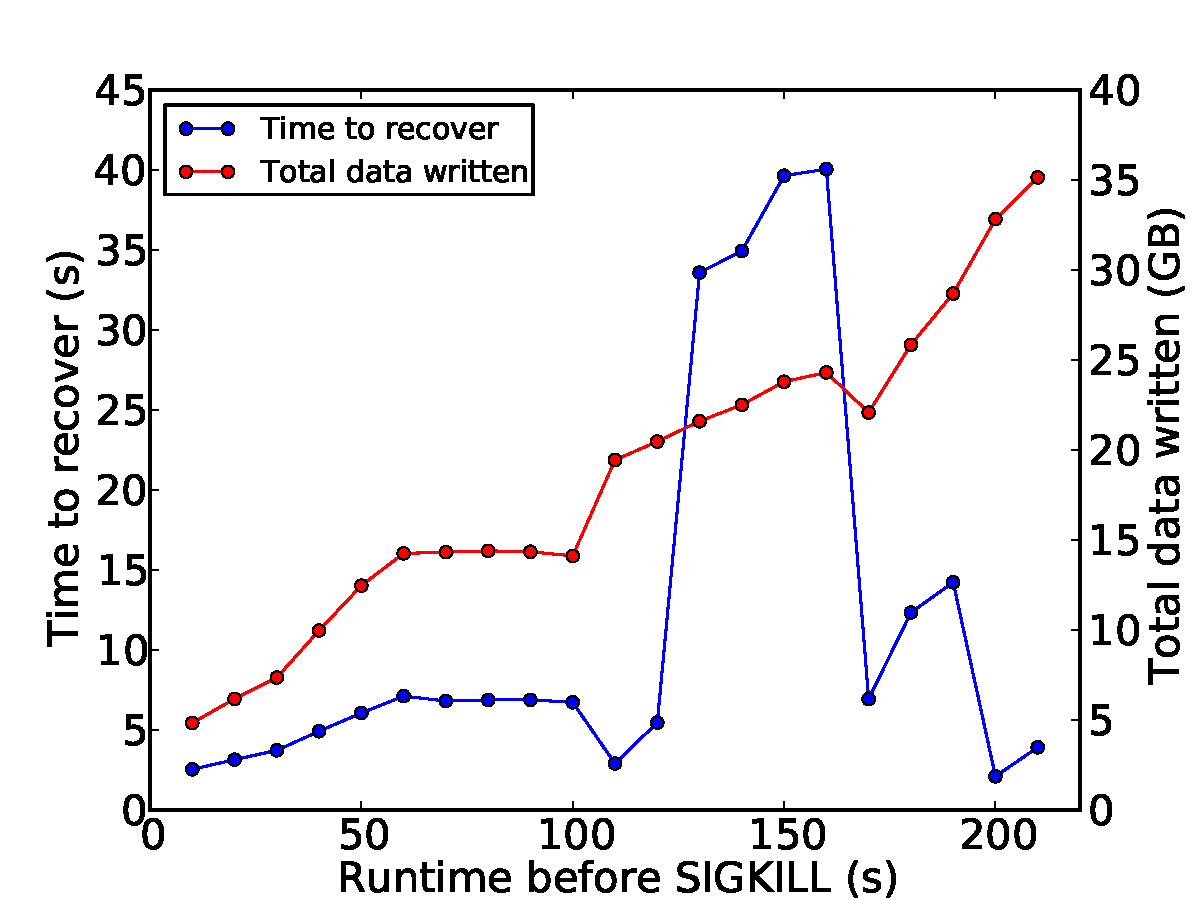
\includegraphics[width=3.5in]{figures/checkpointing.pdf}
   \caption{Recovery time after writing data to LSVD file for a specific amount of time.}
   \label{fig:checkpointing}
\end{figure}

\subsection{File System Benchmarks}
Finally, we measured FreEBS's performance as compared to local disk performance using both microbenchmarks and macrobenchmarks. Results for latency and throughput are presented in Figure \ref{fig:benchmarks}.

\begin{figure}[t!]
  \centering
   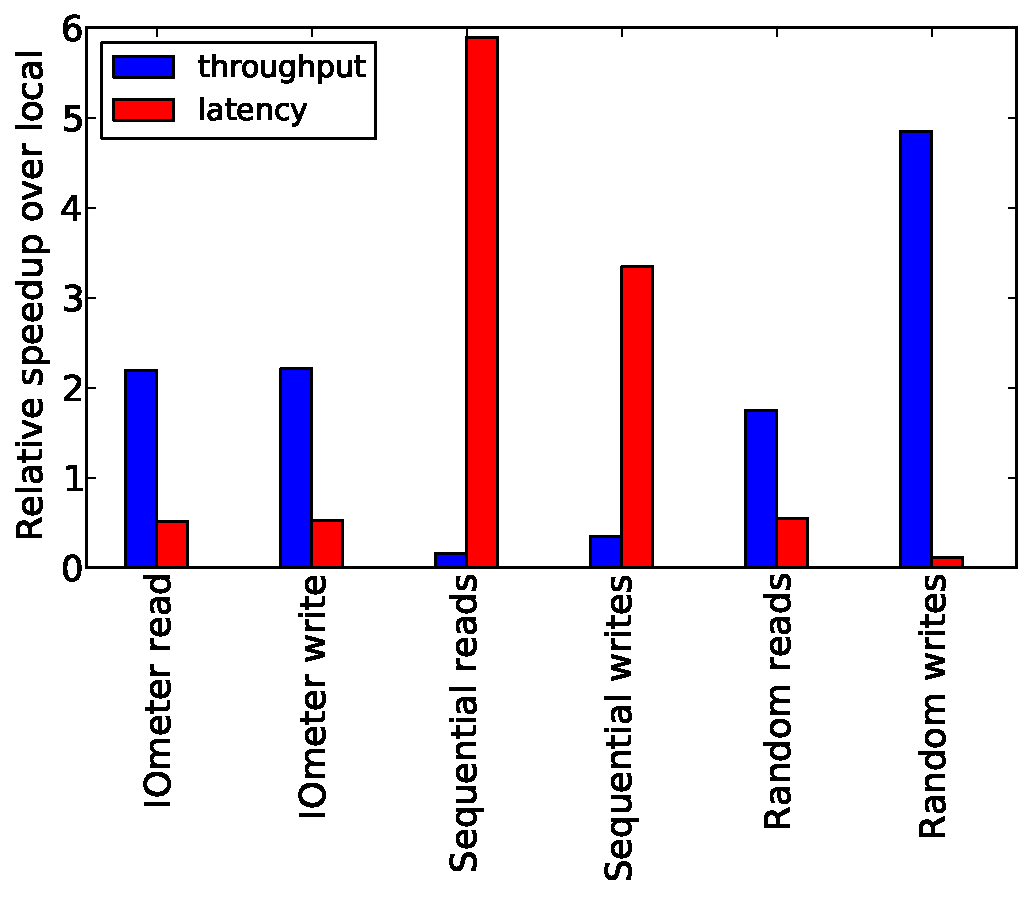
\includegraphics[width=3.5in]{figures/benchmarks.pdf}
   \caption{File system benchmarks.}
   \label{fig:benchmarks}
\end{figure}

The first six benchmarks were run using Flexible IO Tester (fio). The sequential write, sequential read, random write, and random read were run with the synchronous IO engine, which means that operations were conducted with blocking \texttt{read} and \texttt{write} calls. They all used a file size of 256 MB. The sequential benchmarks used block sizes of 4 KB for each operation while the random benchmarks used block sizes of 512 B. The write benchmarks were also configured to issue an \texttt{fsync} call every 128 operations.

The IOMeter benchmark was based on an example configuration included with the fio distribution designed to emulate Intel's IOMeter file server access pattern. It uses libaio (an asynchronous IO library for Linux), an 80\% read/20\% write mix, allows up to 64 requests to be in flight at a given time, and issues requests using a variety of block sizes. We configured it to use a 400 MB file.

Initially, direct I/O was enabled in our benchmarks, but we found that it inflated FreEBS's performance. This is because the replica managers use their local file caches. Since the network was extremely fast, this put the local machine at a disadvantage since it had no cache. Therefore, for all of our benchmarks, we do not use direct I/O.

A final benchmark we ran was to time how long it took to compile the Linux kernel on the volume. For this benchmark, we do not present throughput.

FreEBS excels at random writes due to the log-structured nature of its backing store. It also seems to have done better than local for random reads -- this may be due to the relevant parts of the replica file remaining in cache after setup. Sequential read and write performance is quite bad. This is likely due to the synchronous nature of the tests; every request involves at least one round trip and multiple requests must be serviced serially. The Linux kernel build took twice as long on FreEBS, but this may also be affected by the fact that it was running inside a virtual machine. Further testing could mitigate these problems, but lack of time prevented us from accomplishing this.

After executing random write benchmark, we also evaluated usefulness of LSVD \texttt{cleanup} function. The size of LSVD backing file on primary replica after the benchmark was 2.4GB. Execution of \texttt{cleanup} function reduced the size to 290MB.
